\chapter{MEMORIA DESCRIPTIVA}

\section{Introduccion}

El presente informe desarrolla la propuesta academica de instalaciones electricas interiores para una vivienda unifamiliar de tres niveles ubicada en Jr. Lima S/N, distrito de Capachica, provincia y departamento de Puno. El proyecto corresponde al curso de Instalaciones Electricas I y se formula con criterios de seguridad, funcionalidad, facilidad de mantenimiento y coherencia con el Codigo Nacional de Electricidad -- Utilizacion (CNE-U) y la Norma EM.010 del Reglamento Nacional de Edificaciones.

La propuesta considera suministro monofasico de 220 V, 60 Hz, tablero general, tableros de distribucion, circuitos derivados, canalizaciones empotradas, protecciones termomagneticas y diferenciales, medidor referencial y sistema de puesta a tierra.

\section{Datos generales del proyecto}

\begin{table}[H]
\centering
\small
\caption{Datos generales de la vivienda}
\label{tab:datos-generales-vivienda}
\begin{tabularx}{\textwidth}{L{5.2cm}Y}
\toprule
\textbf{Parametro} & \textbf{Descripcion} \\
\midrule
Propietario & Renzo Gabriel Mamani Galindo \\
Uso & Vivienda unifamiliar \\
Ubicacion & Jr. Lima S/N, Capachica, Puno (Coordenadas: 15°38'32.7''S 69°49'51.8''W) \\
Niveles & Tres niveles \\
Area techada referencial & 120 m2, considerando 40 m2 por nivel \\
Sistema electrico & Monofasico, 220 V, 60 Hz \\
Normas de referencia & CNE-U, RNE EM.010 y NTP aplicables \\
Estado del diseno & Academico preliminar, sujeto a verificacion en obra \\
\bottomrule
\end{tabularx}
\end{table}

\subsection{Ubicación del predio e imágenes catastrales}

El predio se ubica políticamente en el Jirón Lima S/N del distrito de Capachica, provincia y departamento de Puno. Las coordenadas geográficas de referencia son: \textbf{15°38'32.7''S 69°49'51.8''W}.

Para mayor detalle de su emplazamiento, se incorporan a continuación los planos de catastro y vistas de referencia satelital de la vivienda:

\begin{figure}[H]
  \centering
  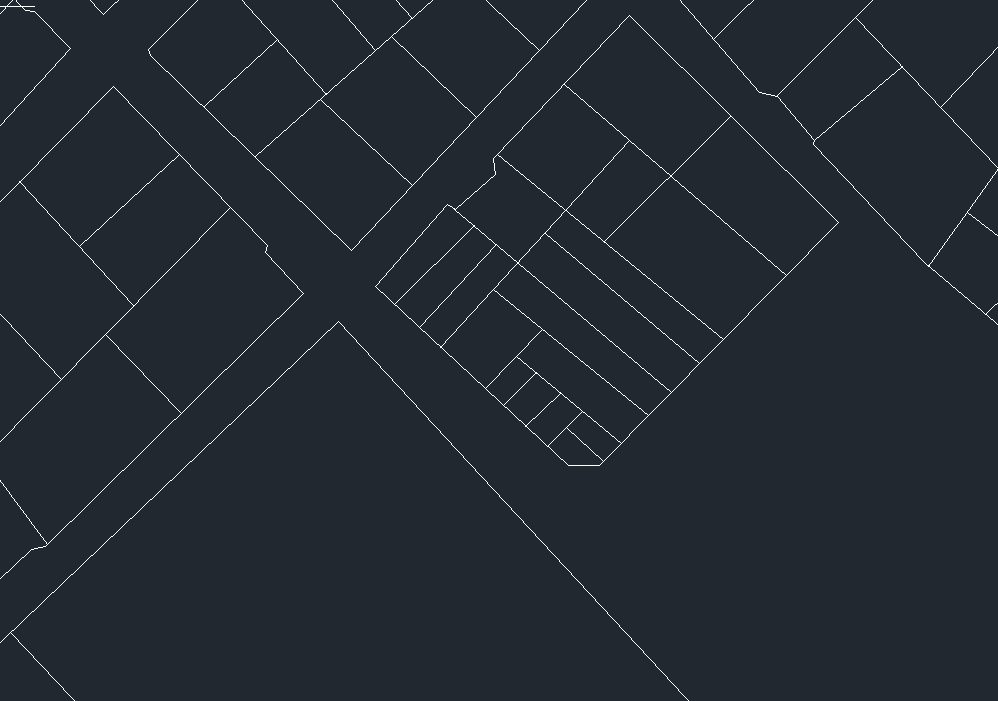
\includegraphics[width=0.85\textwidth]{figuras/plano_catastral.png}
  \caption{Plano Catastral de Ubicación de la Vivienda - Capachica}
  \label{fig:plano-catastral}
\end{figure}

\begin{figure}[H]
  \centering
  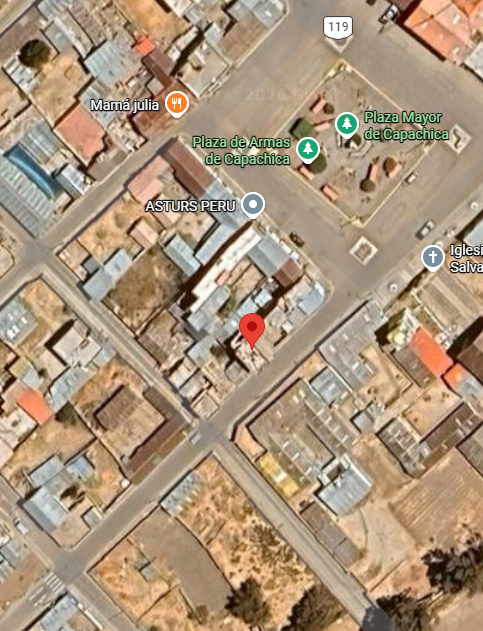
\includegraphics[width=0.85\textwidth]{figuras/ubicacion_satelital.png}
  \caption{Captura Satelital de la Ubicación de la Vivienda (Jr. Lima S/N)}
  \label{fig:ubicacion-satelital}
\end{figure}

\section{Objetivos}

\subsection{Objetivo general}

Desarrollar una propuesta tecnica de instalaciones electricas interiores para la vivienda, integrando memoria descriptiva, calculos justificativos, planos electricos, cuadros de cargas y criterios de seguridad residencial.

\subsection{Objetivos especificos}

\begin{itemize}
  \item Identificar los ambientes funcionales de la vivienda y su distribucion por nivel.
  \item Definir una sectorizacion de circuitos acorde con una vivienda de tres pisos, separando alumbrado y tomacorrientes.
  \item Ubicar luminarias, interruptores, tomacorrientes, y tableros sobre la arquitectura existente.
  \item Dimensionar preliminarmente conductores y dispositivos de proteccion.
  \item Documentar los criterios graficos y tecnicos usados en los planos electricos.
\end{itemize}

\section{Distribucion arquitectonica considerada}

La arquitectura base fue tomada de los planos CAD version 3 generados en el proyecto. Los ambientes reconocidos son los siguientes:

\begin{table}[H]
\centering
\small
\caption{Ambientes reconocidos por nivel}
\label{tab:ambientes-reconocidos}
\begin{tabularx}{\textwidth}{L{2.4cm}Y}
\toprule
\textbf{Nivel} & \textbf{Ambientes considerados} \\
\midrule
Primer piso & Tienda o ambiente frontal, cocina, pasadizo longitudinal y escalera. \\
Segundo piso & Dormitorio principal, dormitorio 3, sala/hall, bano y escalera. \\
Tercer piso & Dormitorio 4, dormitorio 5, pasadizo/vestibulo, bano y escalera. \\
\bottomrule
\end{tabularx}
\end{table}

El ambiente frontal del primer piso se rotula como tienda en el plano arquitectonico. Para efectos electricos se lo considera ambiente de uso frecuente, por lo que se le asignan luminarias y tomacorrientes suficientes para uso social o comercial ligero. Su uso final debe confirmarse en obra.

\section{Criterio de sectorizacion electrica}

Para mejorar la claridad, facilidad de mantenimiento y lectura de planos, se adopta una sectorizacion en 7 circuitos independientes. Cada piso cuenta con un circuito exclusivo para alumbrado (C1, C4, C6) y circuitos exclusivos para tomacorrientes. En el primer piso, se ha independizado el circuito de la cocina (C3) para atender las cargas especiales típicas de dicha área, separándola de los tomacorrientes generales (C2). Se han eliminado circuitos especiales externos para ajustar la instalación exclusivamente al levantamiento real de puntos.

\begin{table}[H]
\centering
\small
\caption{Sectorizacion electrica adoptada}
\label{tab:sectorizacion-adoptada}
\begin{tabularx}{\textwidth}{L{1.4cm}L{4.4cm}Y}
\toprule
\textbf{Circuito} & \textbf{Uso} & \textbf{Criterio} \\
\midrule
C1 & Alumbrado del primer piso & Atiende tienda, cocina, pasadizo y escalera (4 puntos de luz). \\
C2 & Tomacorrientes generales 1er piso & Atiende tienda y pasadizo (5 puntos dobles). \\
C3 & Tomacorrientes de cocina & Atiende puntos especiales de la cocina en el primer piso (3 puntos dobles). \\
C4 & Alumbrado del segundo piso & Atiende dormitorios, hall, bano y escalera (4 puntos de luz). \\
C5 & Tomacorrientes del segundo piso & Atiende dormitorios y sala (8 puntos dobles). \\
C6 & Alumbrado del tercer piso & Atiende dormitorios, pasadizo, bano y escalera (4 puntos de luz). \\
C7 & Tomacorrientes del tercer piso & Atiende dormitorios y bano (6 puntos dobles). \\
\bottomrule
\end{tabularx}
\end{table}

\section{Tableros, medidor y puesta a tierra}

Se propone ubicar el tablero general TG-01 en el primer piso, cerca del ingreso y en zona accesible. El medidor se representa de forma referencial en fachada o ingreso. Por la existencia de tres niveles, se consideran dos tableros de distribucion secundarios: TD-01 asociado al segundo piso y TD-02 asociado al tercer piso.

\begin{itemize}
  \item \textbf{TG-01:} tablero general de corte y proteccion principal del primer piso.
  \item \textbf{TD-01:} tablero de distribucion para el segundo nivel.
  \item \textbf{TD-02:} tablero de distribucion para el tercer nivel.
  \item \textbf{M:} medidor referencial en fachada o zona de ingreso.
  \item \textbf{PT:} puesta a tierra referencial conectada al TG-01.
\end{itemize}

\section{Criterios de ubicacion de puntos}

Los puntos electricos se distribuyen con criterio preliminar sobre los ambientes existentes. Las luminarias se ubican preferentemente al centro de ambientes y se duplican en ambientes alargados o de uso frecuente (como el pasadizo del primer piso y los dormitorios principales). Los interruptores se colocan cerca de accesos, evitando quedar detras de puertas. Los tomacorrientes se distribuyen en muros utiles con conexion a tierra para seguridad del usuario.

\section{Observaciones y datos por confirmar}

\begin{itemize}
  \item Confirmar si el ambiente frontal del primer piso funcionara como tienda, sala o dormitorio.
  \item Confirmar ubicacion definitiva del medidor con la empresa distribuidora.
  \item Confirmar ubicacion final de TG-01, TD-01 y TD-02 en obra.
  \item Verificar recorridos reales de canalizacion antes de ejecutar.
\end{itemize}
